\section{Diagrama de Objetivos (1.1)}

\subsection{Descripci\'on: Preparación}

En la etapa de preparación, el Ministerio provee un listado con los datos personales de todo el padrón, y lo carga en el sistema, junto con el código fuente del mismo, permitiendo así la exposición de los datos a través de la interfaz web. De esta manera, un elector podrá consultar el padrón, y de no figurar en él, se dirigirá al ministerio, donde el sistema le permitirá al ministerio ingresar nuevos votantes  (hasta determinada fecha límite) asignándoles una mesa válida. A su vez, electores, fiscales generales y partidos políticos, podrán revisar el código y ver que no haya ninguna irregularidad en el mismo.

Pasada dicha fecha, el ministerio suministra la información sobre las escuelas disponibles para votar al sistema, y procede a activar la opción “Asignar escuela y mesa” a cada elector, donde el sistema realiza dicha asignación automáticamente. A su vez, asigna de manera aleatoria los presidentes de mesas, ponderando a los que nunca lo fueron previamente.\\

Dado que el ministerio precisa conocer a los presidentes de mesa designados, el sistema permite consultar quienes son los mismos, de manera que el Ministerio pueda comunicarse con ellos. En caso de que algún notificado no pudiera estar presente (con justificación válida), el sistema permitirá al Ministerio elegir uno nuevo. Quedará a cargo del Ministerio, la capacitación de los mismos.\\

Posteriormente, los partidos políticos presentan sus candidatos al Ministerio (hasta determinada fecha límite). Pasada la misma, el Ministerio carga esta información en la versión Web para que esté disponible a consultar y el equipo técnico del mismo graba la información en las máquinas impresoras de voto. En este momento, también, asigna una máquina impresora de voto a cada mesa, más dos extra por escuela (en caso de que suceda algún exabrupto), sumado a una máquina extra (que sólo será utilizada para el envío de datos de resultados) y un cable de conexión de teléfono. Cada máquina posee una batería que dura 3 hs sin estar conectada a alimentación eléctrica. El sistema proveerá una contraseña única para todas las máquinas para entrar en el “Modo envío” y ademas una contraseña única por Fiscal General de escuela, los cuales se utilizarán en el momento de cargar los resultados de la elección.\\

Luego, se prepara un lote de boletas para cada mesa, considerando entre ellas a la boleta donde se imprimirán los resultados. Por cada mesa, se asignan además una cantidad extra de boletas, en caso de que algún votante termine utilizando más de una (dado que se puede arrepentir antes de efectuar su voto). Las boletas tienen dos troqueles iguales, los cuales permiten identificar que la misma no fue intercambiada por el votante al momento de realizar la elección, evitando así este tipo de fraude. Las mismas tienen un espacio para impresión con tinta, y un chip grabable dentro.\\

Después, el Ministerio imprime copias del padrón correspondiente a cada mesa, para que sean utilizados por los presidentes de mesa, fiscales y las escuelas, estas mismas lo deberán dejar en un lugar visible para que los votantes puedan consultarlo. También prepara las urnas, armando tantas como cantidad de mesas haya, las cuales poseen una identificación de la mesa a la que pertenecen; y provee un par de auriculares para cada escuela, que recibirán los encargados de las mismas, los cuales brindarán a los votantes no videntes una ayuda a la hora del sufragio. Es el ministerio también el encargado de entregarle a cada Fiscal General las dos contraseñas, \textcolor{red}{y un pendrive que se insertará en las máquinas, para veríficar que el checksum sea correcto.}

Una vez está todo preparado, el Ministerio notifica a las fuerzas de seguridad las escuelas seleccionadas para la elección donde deberán brindar aporte.\\

Llegado el dia de la elección, el correo lleva a cada escuela correspondiente, la cantidad de máquinas de voto asignadas junto a las máquinas extra, todas con sus baterías correspondientes. Además, lleva las boletas, las urnas, las copias del padrón y los auriculares. Todo esto es recibido por el encargado, quien se los otorgará a los presidente de mesa y fiscales. Una vez allí, el fiscal general junto a los presidentes de mesa que ya estén presentes y las fuerzas de seguridad, distribuyen una mesa por aula. A su vez, se posicionan las urnas, las boletas y las máquinas de votación en su lugar correspondiente. El par de auriculares permanecerá en posesión del Fiscal General, quien será el encargado de otorgarlo de ser necesario.

Cada presidente de mesa se ubica en su mesa respectiva. Si llega un votante a una mesa, y esta no cuenta con un presidente de mesa, el fiscal general de la escuela lo nombrará como presidente de dicha mesa. Cada presidente de mesa da inicio a la votación. Lo hace al activar una opción en la máquina de votación. El presidente de mesa es quien emitirá su voto primero acorde a lo explicado posteriormente. A partir de ese momento, cualquier votante habilitado que llegue a su mesa podrá emitir sufragio.

\newpage
\subsection{Diagrama}

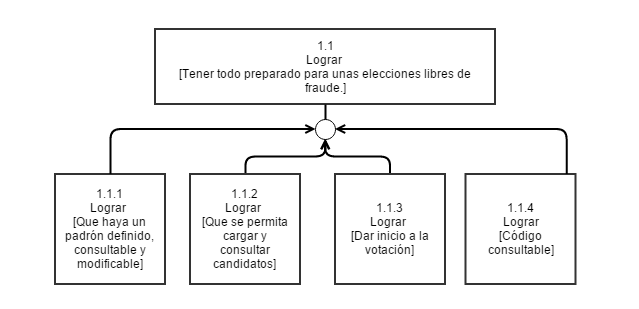
\includegraphics[scale=0.55]{imagenes/Diagramas/11/11.png}
\\
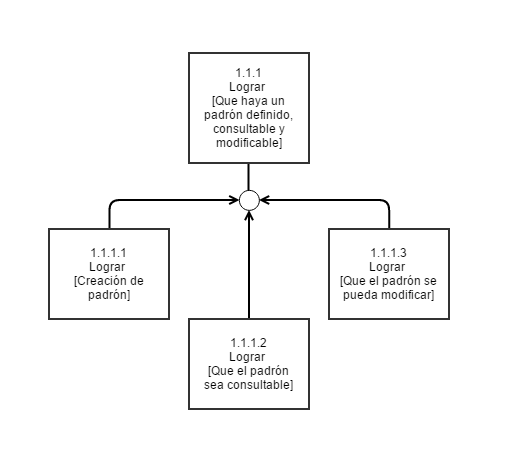
\includegraphics[scale=0.55]{imagenes/Diagramas/11/111.png}
\\
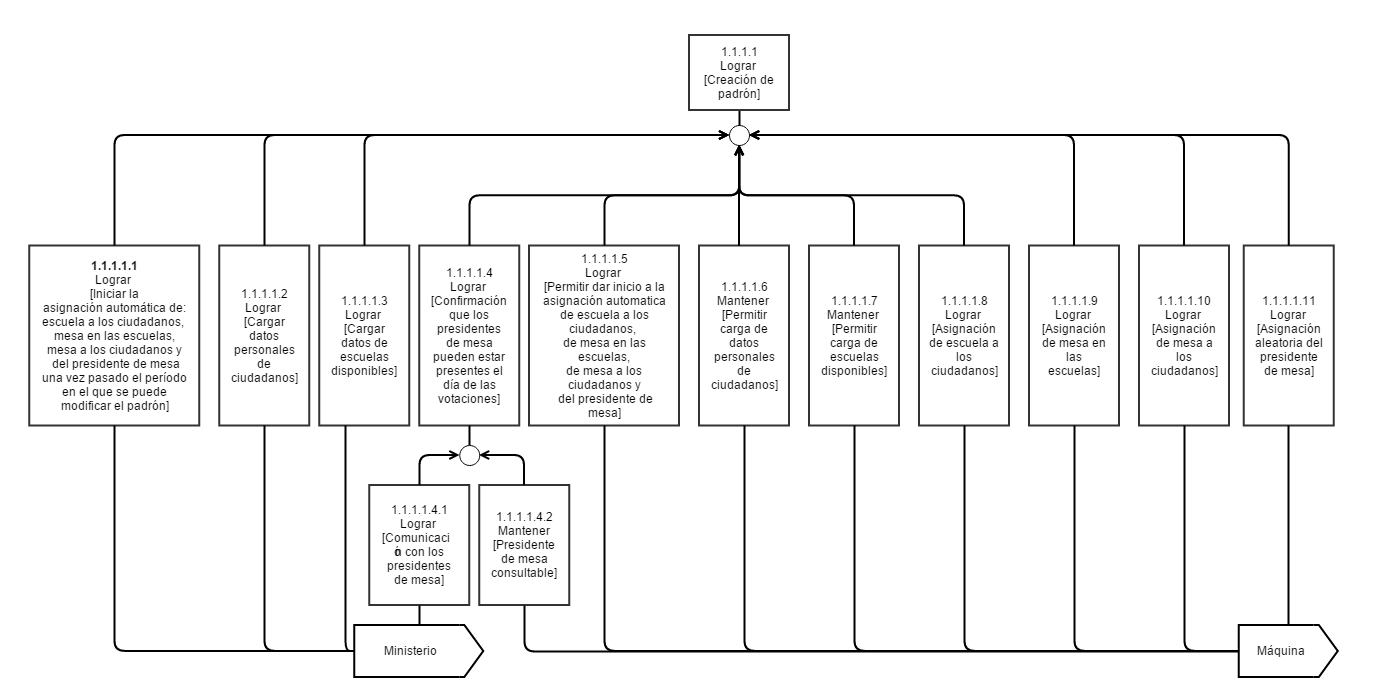
\includegraphics[scale=0.45]{imagenes/Diagramas/11/1111.png}
\\
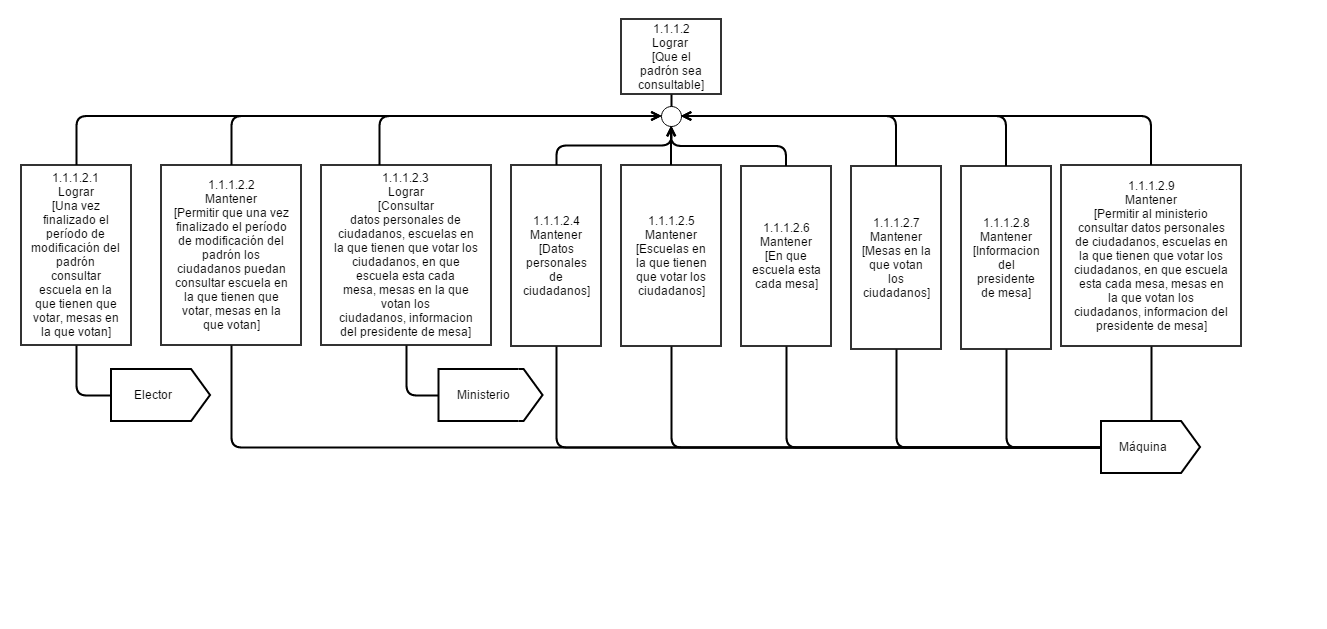
\includegraphics[scale=0.54]{imagenes/Diagramas/11/1112.png}
\\
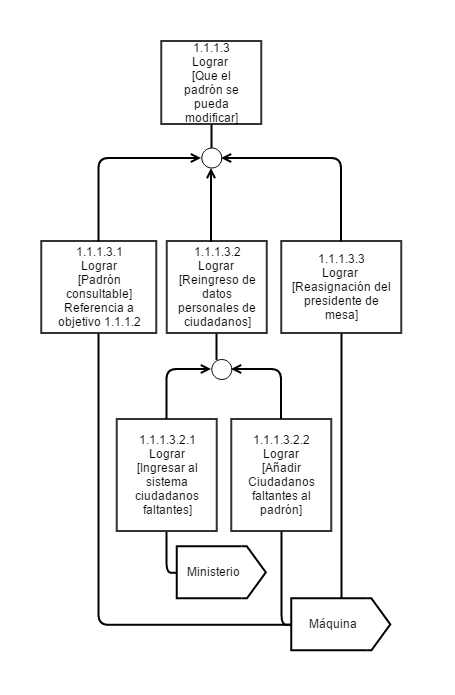
\includegraphics[scale=0.55]{imagenes/Diagramas/11/1113.png}
\\
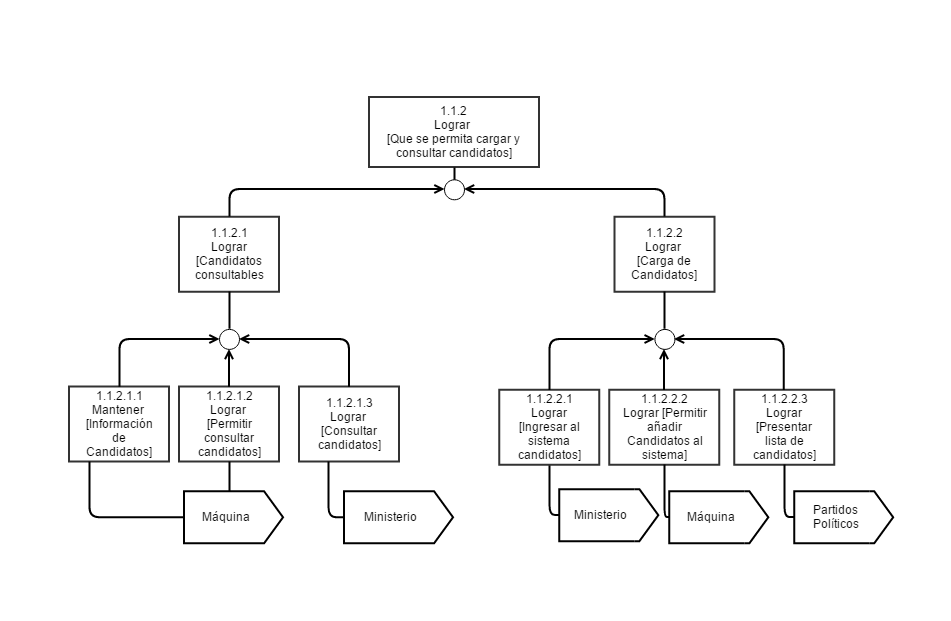
\includegraphics[scale=0.55]{imagenes/Diagramas/11/112.png}
\\
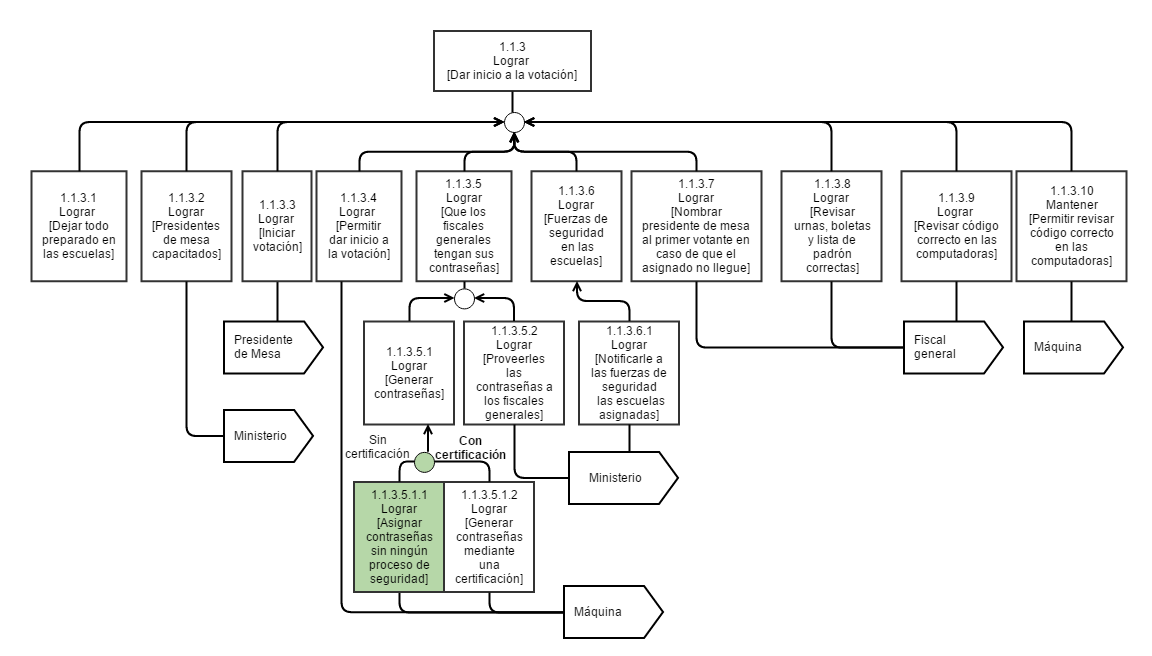
\includegraphics[scale=0.55]{imagenes/Diagramas/11/113.png}
\\
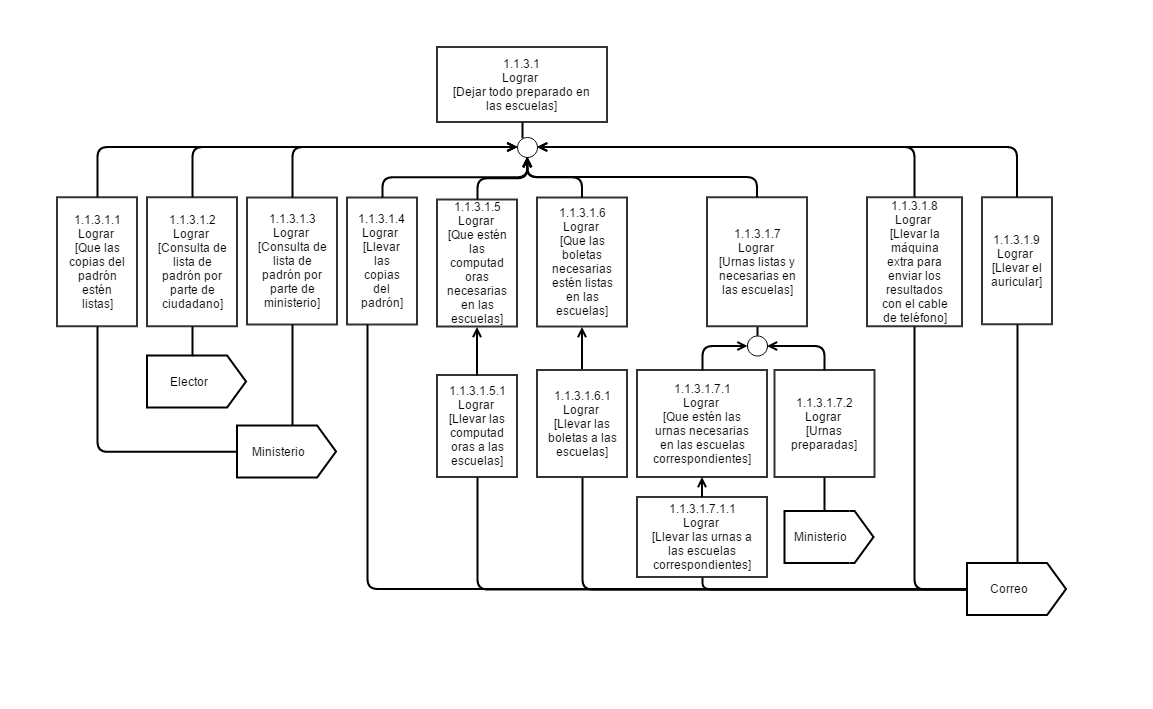
\includegraphics[scale=0.55]{imagenes/Diagramas/11/1131a.png}
\\
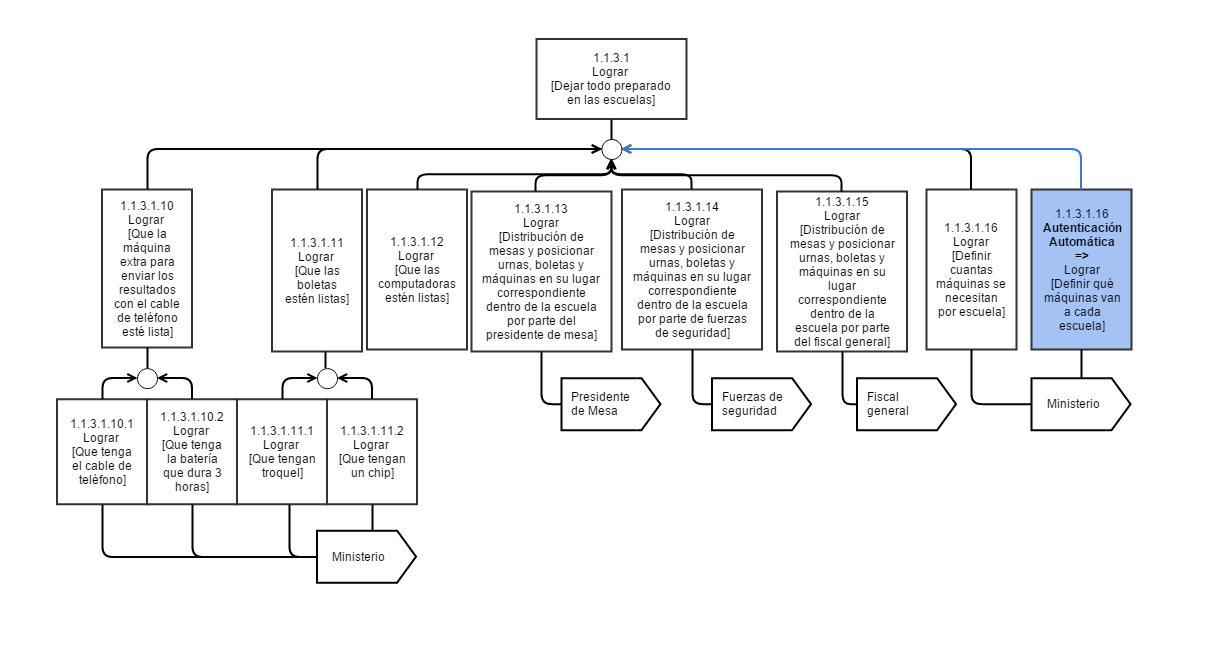
\includegraphics[scale=0.55]{imagenes/Diagramas/11/1131b.png}
\\
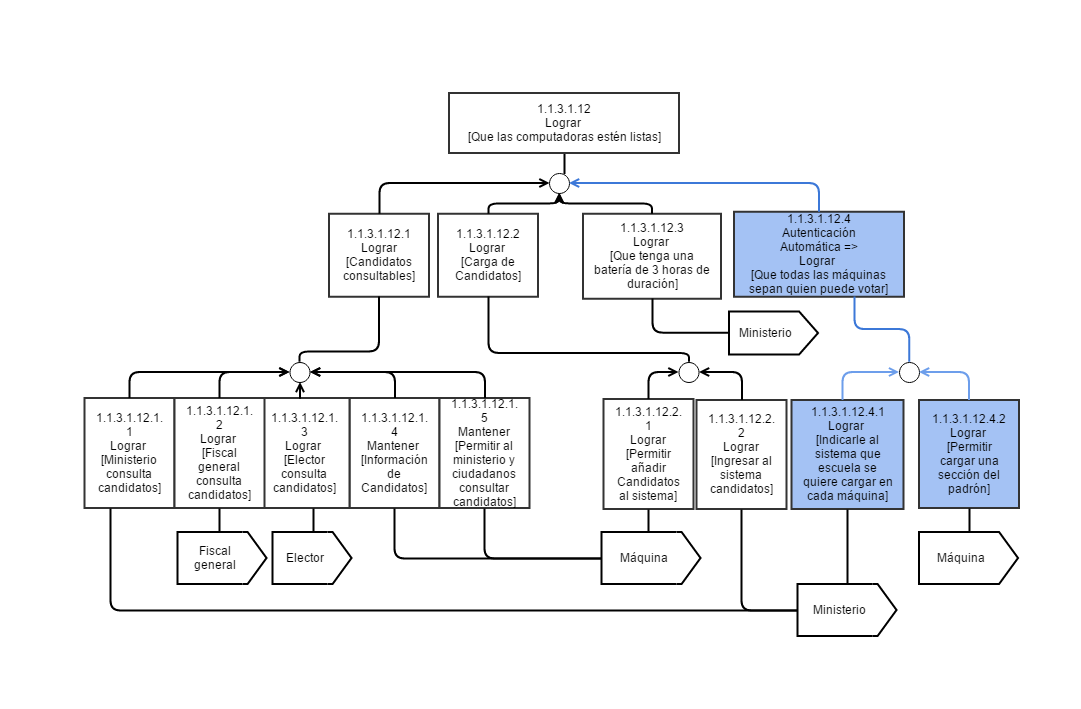
\includegraphics[scale=0.55]{imagenes/Diagramas/11/113112.png}
\\
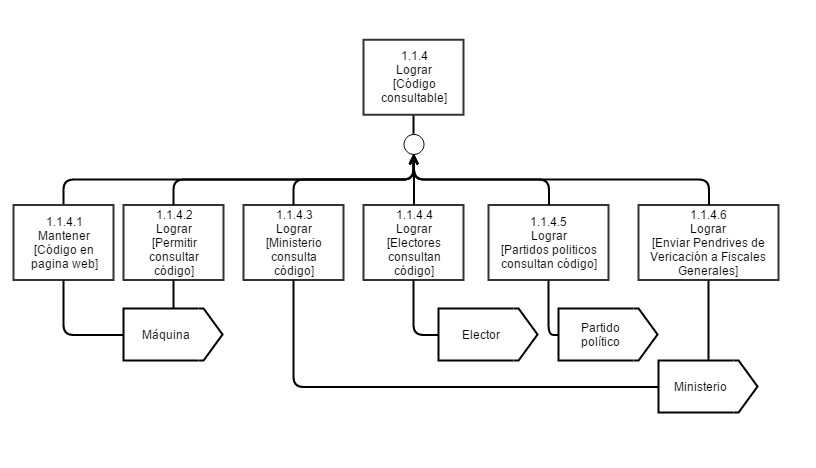
\includegraphics[scale=0.55]{imagenes/Diagramas/11/114.png}




\newpage
\subsection{Lista de requerimientos}

Dado el diagrama de objetivos, podemos rescatar de él un conjunto de requerimientos para 
nuestro sistema. Especificamente todos los objetivos que tengan como agente a la 
\textit{máquina} serán parte del listado de requerimientos de nuestro software.\\


Presentamos a continuación los requerimientos que se decantan de esta sección del diagrama de 
objetivos:

\begin{itemize}
\item Permitir asignación automatica de escuela y mesa a los ciudadanos
\item Permitir asignación de presidente de mesa
\item Permitir la carga de datos personales de ciudadanos
\item Permitir carga de escuelas disponibles
\item Asignar aleatoriamente presidente de mesa
\item Permitir que una vez finalizado el período de modificación del padrón los ciudadanos puedan consultar escuela en la que tienen que votar, mesas en la que votan
\item Permitir al ministerio consultar datos personales de ciudadanos, escuelas en la que tienen que votar los ciudadanos, en que escuela esta cada mesa, mesas en la que votan los ciudadanos, informacion del presidente de mesa
\item Permitir padrón consultable
\item Permitir añadir ciudadanos faltantes al padrón
\item Permitir reasignar presidente de mesa
\item Permitir consultar cantidatos
\item Permitir añadir candidatos al sistema
\item Generar contraseñas para fiscales generales 
\item Permitir revisar código
\item Mostrar código en web
\item Permitir código consultable
\item Permitir revisar código correcto en las computadoras

\end{itemize}
